\subsection{Erklärbares maschinelles Lernen}
\label{subsec:XAI}
Erklärbares maschinelles Lernen (engl.: \emph{Explainable Artificial Intelligence}; Abkz.: XAI) hat zum Gegenstand Systeme künstlicher Intelligenz zu schaffen, welche Vorhersagen erklären können \cite{xu2019explainable, sheh2018defining}.
Unter dem Begriff \enquote{Erklären} wird grundsätzlich das Abgeben eines Grundes oder einer Rechtfertigung für eine gewisse Handlung verstanden \cite{doran2017does}. Insbesondere bei selbstlernenden Systemen, welche in der Medizin oder bei der Klassifikation von Menschen eingesetzt werden (und dabei eventuell unethische Entscheidungen treffen könnten), ist es verständlich, dass Nutzer getroffene Systementscheidungen nachvollziehen wollen oder müssen \cite{antoniadi2021current, xu2019explainable}. Aber nicht nur für Nutzer ist es von Vorteil ML-Systeme zu verstehen; auch Entwicklern wird es leichter fallen, das Potenzial des Systems voll auszuschöpfen, wenn sie die Entscheidungen des ML-Algorithmus nachvollziehen können \cite{xu2019explainable}. So stellt XAI speziell bei neuronalen Netzen, wie CNNs oder RNNs einen Mehrwert bereit, da diese durch ihre häufig vielen Neuronen und Verbindungen als besonders undurchdringbare Blackboxen wirken \cite{xu2019explainable, Ng.2018}.

\subsubsection{Erkläransätze}
\label{subsubsec:Erklaeransaetze}
Um diese Blackboxen zu erklären, existieren mehrere grundlegende Ansätze, von denen sich einige eher an den Entwicklern, andere wiederum an den Nutzern eines Systems orientieren \cite{xu2019explainable}. \cite{kamath2021explainable} untergliedern die Methoden der XAI in drei Kategorien: \emph{Umfang}, \emph{Stadium} und \emph{Modell}. Steht der Umfang im Vordergrund, lassen sich lokale oder globale Methoden anwenden, um ein ML-System zu erklären. Globale Erklärmethoden agieren auf Makroebene und versuchen, die Vorhersagen des Gesamtmodells zu erklären, wobei vor allem ein grobes Verständnis über die Strukturen und Parameter geschaffen werden soll. Lokale Erklärungsansätze hingegen beziehen sich auf konkrete Vorhersagen, indem dargelegt wird, worauf eine bestimmte Vorhersage beruht. Dies könnte z.B. ein konkreter Gegenstand sein, welcher auf einem Bild zu sehen ist \cite{kamath2021explainable}.

\begin{figure}
    \centering
    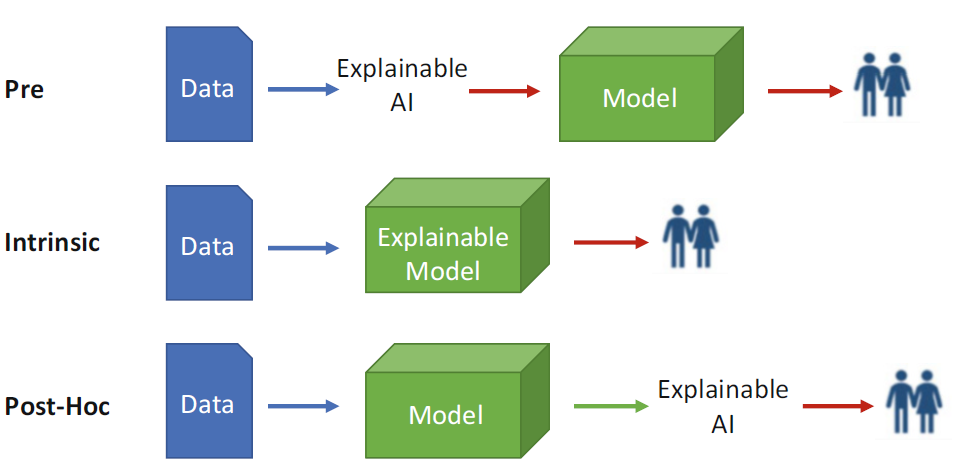
\includegraphics[scale=0.6]{pic/MA-Bilder/explainableAIStages.PNG}
    \caption{XAI Methoden nach Stadium, entnommen aus \cite{kamath2021explainable}}
    \label{Fig:AIMethoden_nach_Stage}
\end{figure}%
Methoden der XAI lassen sich überdies dahingehend unterscheiden, in welchem Stadium diese eingesetzt werden, was in Abbildung \ref{Fig:AIMethoden_nach_Stage} illustriert ist. Hierbei wird zwischen \emph{Pre-Model}, \emph{Intrinsic} oder \emph{Post-Hoc} differenziert. Ansätze, welche sich den Pre-Model-Methoden zuordnen lassen, finden vor der eigentlichen Modellauswahl statt. Daher liegt hier der Fokus nicht auf einem konkreten Modell, sondern auf den zugrundeliegenden Daten. Aktivitäten, welche im Rahmen von Pre-Model-Erklärungsansätzen durchgeführt werden können, sind z.B. das Verstehen, die Auswahl oder die Reduzierung der Daten. Bei der Anwendung intrinsischer Erklärmethoden, machen sich Entwickler die selbsterklärende Struktur einiger ML-Algorithmen zunutze, wie sie z.B. Entscheidungsbäume besitzen. Angemerkt sei an dieser Stelle, dass diese Art der Methode etwas eingeschränkt ist, da nicht jeder Algorithmus eine solche Struktur für Erklärungen mit sich bringt. Post-Hoc-Methoden als dritte Art der Unterscheidung füllen diese Lücke, da sie sich auf Blackbox-Systeme anwenden lassen können. Indem Beziehungen zwischen den Eingabewerten und Vorhersagen verdeutlicht werden, lässt sich auch das Verhalten von Modellen erklären \cite{kamath2021explainable}. Diese Methoden fokussieren sich eher auf den Nutzer und können z.B. mittels Visualisierungen oder Beispielen aus den Trainingsdaten die Entscheidungen des Algorithmus untermauern \cite{xu2019explainable}. Ein besonderer Vorteil der Post-Hoc-Methoden besteht darin, dass es nicht zwingend notwendig ist, die interne Struktur des ML-Systems in Gänze zu kennen oder zu verstehen \cite{kamath2021explainable}. 

Schlussendlich lassen sich Erklärungsansätze entweder als \enquote{Modelagnostic} oder als \enquote{Modelspecific} bezeichnen. Während Erkläransätze existieren, welche sich auf jedes Modell anwenden lassen (Modelagnostic), gibt es auch spezielle Methoden, die nur für bestimmte Typen von ML-Algortihmen geeignet sind (Modelspecific) \cite{kamath2021explainable}.

\subsubsection{Erklärungen}
Mithilfe der im vorangegangen Kapitel \ref{subsubsec:Erklaeransaetze} erläuterten Ansätzen, lassen sich verschiedene Erklärungen für das Verhalten eines ML-Algortihmus erstellen. \cite{kamath2021explainable} nennen \emph{globale}, \emph{lokale}, \emph{kontrastive}, \emph{Was-wäre-wenn}, \emph{kontrafaktische} und \emph{beispielbasierte Erklärungen} auf welche im folgenden näher eingegangen wird.

Globale Erklärungen sind ganzheitliche top-down-Ansätze und fokussieren sich auf die Funktionsweise des Modells, welche mit Visualisierungen, mathematischen Formeln oder Graphen abgebildet werden kann. Während globale Erklärungen, darlegen, wie ein Modell funktioniert, bilden lokale Erklärungen als bottom-up-Ansätze eher ab, wieso ein Modell eine bestimmte Entscheidung getroffen hat. Ähnlich dazu können im XAI-Umfeld kontrastive Erklärungen abgegeben werden, die Aussagen der Form \enquote{Warum X und warum nicht Y} treffen. Diese eignen sich besonders dazu, Auswirkungen von minimalen Änderungen einzelner Modellparameter zu analysieren. \enquote{Was-wäre-wenn}-Erklärungen legen wiederum da, wie sich ein Modell bei Änderung bestimmter Eingaben oder Parameter verändern würden und schaffen somit Verständnis dafür, wie Vorhersagen und Parameter zueinander in Beziehungen stehen. Ähnlich dazu wirken kontrafaktische Erklärungen, die angeben, welche Änderungen am Modell zu welchen anderen Ausgaben führen würden. Somit bekommen Entwickler eine Idee davon, wie sich ein gewünschtes Ergebnis mit minimalen Änderungen erreichen ließe. Eine simple Art der Erklärung besteht darin Beispiele mitzugeben, welche aus den Trainingsdaten stammen \cite{kamath2021explainable}.

 Von diesen bis zu dieser Stelle eher abstrakt umrissenen Erklärung(-sansätzen) existieren konkrete Instanzen, welche ML erklärbar machen. Ein bekanntes Beispiel ist \enquote{Local Interpretable Model-Agnostic Explanations} (LIME), welches sich für mehrere Arten von Klassifikationsverfahren einsetzen lässt \cite{ribeiro2016should}. Aufgrund ihrer Nicht-Interpetierbarkeit stehen DL-Netzwerke jedoch besonders im Vordergrund des XAI-Forschungsfeldes \cite{holzinger2018machine}. Für diese ML-Typen existieren Verfahren, die z.B. anzeigen, welche Neuronen besonders stark aktivierte wurden. Hiervon wird sich erhofft, Rückschlüsse darauf zu ziehen, welches Merkmal besonders wichtig ist \cite{xu2019explainable}. Eine weitere konkrete Methode heißt \enquote{Layer-Wise Relevance Propagation}, welche Werte für die Relevanz eines Neurons für das Zustandekommen einer bestimmten Entscheidung ermitteln kann. Hier wird der Lernprozess rückwärts durchlaufen und so kann ermittelt werden, welches Neuronen welchen Beitrag für die Entscheidung beigetragen hatte \cite{montavon2019layer}.
Auf weitere konkrete Methoden wird in Kapitel \todo{tbd} im Rahmen der Handreichung eingegangen.